\documentclass[9pt,pdftex]{beamer}

% use git: import repository as new project in eclipse: http://www.eclipse.org/forums/index.php/t/226301/

\usepackage[utf8]{inputenc}
\usepackage[english]{babel}
\usepackage{amsfonts, amsmath, amssymb}
\usepackage{color}
\usepackage{fancybox}
\usepackage{graphicx}
\usepackage{multirow}
% \usepackage{paralist}
\usepackage{todonotes}
%\usepackage{biblatex}
\usepackage{subfig}
\newenvironment{figure*}%
{\begin{figure}}
{\end{figure}}

\usepackage{hyperref}

%\usepackage[style=mla,babel=hyphen,backend=biber]{biblatex}

% CSE-Beamer-Styles:
%\usepackage[conference]{beamertheme_sccstalk}
\usepackage[lecture]{beamertheme_sccstalk}
\usepackage{beamercolorscheme_sccs}
\usepackage{beamerfontthemestructurebold}

\graphicspath{{img/}}

\setcounter{tocdepth}{3} 

\title{Simulation of the air flow in the MI building with LBM}
\subtitle{CFD Lab Project: midterm presentation}
\author[Group 2]{Group 2: Martin Andreev, Gerasimos Chourdakis, Igor Tominec \\ Advisor: Kaveh Rahnema} %[displayed in footer]{displayed on title page}
\date{July 17th, 2015}
\institute{Technische Universität München}

\begin{document}
	\frame{\titlepage}

	%===========================================================================
\section*{Contents}
\begin{frame}{Contents}
\tableofcontents
\end{frame}
	
%===========================================================================

\section{The idea}
\begin{frame}{The idea}
 \begin{itemize}
  \item Parallel approach for arbitrary geometries.
  \item Do not waste effort for large ``inactive'' areas.
%   \item Use the Lattice Boltzmann Method (BGK LBM).
  \item Case study: Mathematics-Informatics building-like geometry. 
 \end{itemize}
\end{frame}


\section{The model}

\begin{frame}{Real life}
\begin{figure}
\includegraphics[width=0.8\linewidth]{MI_slides}
\end{figure}
\end{frame}

\begin{frame}{Approximation}
\only<1>{\begin{figure}\includegraphics[width=0.8\linewidth]{MI_slides_verylow}\end{figure}}
\only<2>{\begin{figure}\includegraphics[width=0.8\linewidth]{MI_slides_mario_f1}\end{figure}}
\only<3>{\begin{figure}\includegraphics[width=0.8\linewidth]{MI_slides_mario_f2}\end{figure}}
\only<4>{\begin{figure}\includegraphics[width=0.8\linewidth]{MI_slides_mario_f3}\end{figure}}
\only<5>{\begin{figure}\includegraphics[width=0.8\linewidth]{MI_slides_mario_f4}\end{figure}}
\only<6>{\begin{figure}\includegraphics[width=0.8\linewidth]{MI_slides_mario_f5}\end{figure}}
\end{frame}

\begin{frame}{The model}
 \begin{itemize}
  \item Real life
  \begin{itemize}
   \item Main hall: approx. 150m long, 12-26m wide (mean: 19m).
   \item Wings: approx. 10m long, 40-50m wide.
   \item Mass, momentum and heat transfer laws in 3D.
   \item Flow due to pressure and density differencies.
   \item Air with very low speed.
   \item Doors mainly closed.
  \end{itemize}
  
  \pause
  
  \item Model
  \begin{itemize}
   \item Main hall: rectangle, 16$x$ long, 2$x$ wide (ratio 16:2).
   \item Wings: rectangles, 1$x$ long, 4$x$ wide (ratio 1:4).
   \item LBM with BGK approximation in pseudo-3D (2D).
   \item Flow due to constant inflow velocities.
   \item BGK-compatible relaxation time ($\tau$ parameter).
   \item Larger doors, always (or randomly) open.
  \end{itemize}

 \end{itemize}
\end{frame}

\begin{frame}{The geometry}
The geometry (pgm files of flagfield) is produced in Matlab, for given x.
Various boundary conditions and obstacles can be defined.
 \begin{figure}
  \includegraphics[width=0.8\linewidth]{matlab_whole_domain}
 \end{figure}
\end{frame}

\section{Partitioning}
\begin{frame}{Partitioning: Worksheet 4 - style}
 Let's divide the geometry in 4 parts intuitively:
 \begin{figure}
  \includegraphics[width=0.8\linewidth]{matlab_domain_WS4}
 \end{figure}
 Total area: 160$x^2$\pause, active area: 72$x^2$ (45\%) \pause, inactive area: 88$x^2$ (55\%).
\end{frame}

\begin{frame}{Partitioning: our approach}
 Try to eliminate the inactive area:
 \begin{figure}
  \includegraphics[width=0.8\linewidth]{actual_partitioning_sizes}
 \end{figure}
 Total area: 72$x^2$, active area: 72$x^2$ (100\%) - approximately.
\end{frame}

\section{Work balance}
\begin{frame}{Distribution to CPUs}
 Each process (we assume np=8) is assigned one or more partitions-chunks in order to
 keep the work balanced. All the chunks are stored in the same array, with known offsets. 
 \begin{figure}
  \includegraphics[width=0.8\linewidth]{cpus_divided}
 \end{figure}

\end{frame}

\begin{frame}{Work balance}
 With the proposed partitioning and distribution, each process is assigned
 with 8$x^2$ lattice cells in the normal case, or 12$x^2$ in the worst case,
 including no large inactive areas.
 \begin{figure}
  \includegraphics[width=0.8\linewidth]{load_balance}
 \end{figure} 
\end{frame}

\section{Communication}
\begin{frame}{Communication}
  Every process has to communicate with one or more
  neighbors, for one or more partitions. Every process knows:
  \begin{itemize}
   \item the ids of the chunks it has to process,
   \item the neighboring processes (number and ids) and chunks.
  \end{itemize}
  The processes communicate asynchronously, waiting for the whole communication to complete.
 \begin{figure}
  \includegraphics[width=0.6\linewidth]{cpus_divided_chunks}
 \end{figure} 
\end{frame}

\section{Implementation}
\begin{frame}{What we did}
 Main tasks:
 \begin{itemize}
  \item Physical geometry definition (measurements)
  \item Problem geometry definition (well separable)
  \item \textbf{Domain partitioning}
  \item \textbf{(Automated) geometry files creation}
  \item Work scheduling
  \item Generalization of the WS3 code (multiple inlets)
  \item Randomly opening doors
  \item Merging of WS3 and WS4
  \item \textbf{Definition of chunks, offsets, neighbors}
  \item \textbf{Communication for multiple neighbors and chunks}
  \item Visualization of multiple chunks
  \pause
  \item \textbf{Much much much debugging...}
 \end{itemize}
\end{frame}

\section{Results}
 \begin{frame}{Results}
  Grab your popcorn, it's movie time!
 \end{frame}
 
 \begin{frame}{Results (example)}
  For those who slept during the movie, this is an example timestep of
  our simulation, with $\tau=0.6$, inlets with perpendicular velocity = 0.1 and $x=16$ lattice cells.
  The color shows the velocity magnitude. %As the parameters are unphysical, the actual values are ommitted.
  \begin{figure}
   \includegraphics[width=0.8\linewidth]{results_3inlets_streamlines}
  \end{figure}
 \end{frame}
 
 \begin{frame}{Thank you!}
  It is hot today! We understand you and thanks for the attention!
  \vspace{1cm}
  
  Find our work on GitHub: \href{https://github.com/MakisH/CFDLab}{\url{github.com/MakisH/CFDLab}} \\
  (expect some rough edges)
  
 \end{frame}



 







\end{document}
